
%% bare_conf.tex
%% V1.4b
%% 2015/08/26
%% by Michael Shell
%% See:
%% http://www.michaelshell.org/
%% for current contact information.
%%
%% This is a skeleton file demonstrating the use of IEEEtran.cls
%% (requires IEEEtran.cls version 1.8b or later) with an IEEE
%% conference paper.
%%
%% Support sites:
%% http://www.michaelshell.org/tex/ieeetran/
%% http://www.ctan.org/pkg/ieeetran
%% and
%% http://www.ieee.org/

%%*************************************************************************
%% Legal Notice:
%% This code is offered as-is without any warranty either expressed or
%% implied; without even the implied warranty of MERCHANTABILITY or
%% FITNESS FOR A PARTICULAR PURPOSE! 
%% User assumes all risk.
%% In no event shall the IEEE or any contributor to this code be liable for
%% any damages or losses, including, but not limited to, incidental,
%% consequential, or any other damages, resulting from the use or misuse
%% of any information contained here.
%%
%% All comments are the opinions of their respective authors and are not
%% necessarily endorsed by the IEEE.
%%
%% This work is distributed under the LaTeX Project Public License (LPPL)
%% ( http://www.latex-project.org/ ) version 1.3, and may be freely used,
%% distributed and modified. A copy of the LPPL, version 1.3, is included
%% in the base LaTeX documentation of all distributions of LaTeX released
%% 2003/12/01 or later.
%% Retain all contribution notices and credits.
%% ** Modified files should be clearly indicated as such, including  **
%% ** renaming them and changing author support contact information. **
%%*************************************************************************


% *** Authors should verify (and, if needed, correct) their LaTeX system  ***
% *** with the testflow diagnostic prior to trusting their LaTeX platform ***
% *** with production work. The IEEE's font choices and paper sizes can   ***
% *** trigger bugs that do not appear when using other class files.       ***                          ***
% The testflow support page is at:
% http://www.michaelshell.org/tex/testflow/



\documentclass[conference]{IEEEtran}
% Some Computer Society conferences also require the compsoc mode option,
% but others use the standard conference format.
%
% If IEEEtran.cls has not been installed into the LaTeX system files,
% manually specify the path to it like:
% \documentclass[conference]{../sty/IEEEtran}





% Some very useful LaTeX packages include:
% (uncomment the ones you want to load)


% *** MISC UTILITY PACKAGES ***
%
%\usepackage{ifpdf}
% Heiko Oberdiek's ifpdf.sty is very useful if you need conditional
% compilation based on whether the output is pdf or dvi.
% usage:
% \ifpdf
%   % pdf code
% \else
%   % dvi code
% \fi
% The latest version of ifpdf.sty can be obtained from:
% http://www.ctan.org/pkg/ifpdf
% Also, note that IEEEtran.cls V1.7 and later provides a builtin
% \ifCLASSINFOpdf conditional that works the same way.
% When switching from latex to pdflatex and vice-versa, the compiler may
% have to be run twice to clear warning/error messages.






% *** CITATION PACKAGES ***
%
%\usepackage{cite}
% cite.sty was written by Donald Arseneau
% V1.6 and later of IEEEtran pre-defines the format of the cite.sty package
% \cite{} output to follow that of the IEEE. Loading the cite package will
% result in citation numbers being automatically sorted and properly
% "compressed/ranged". e.g., [1], [9], [2], [7], [5], [6] without using
% cite.sty will become [1], [2], [5]--[7], [9] using cite.sty. cite.sty's
% \cite will automatically add leading space, if needed. Use cite.sty's
% noadjust option (cite.sty V3.8 and later) if you want to turn this off
% such as if a citation ever needs to be enclosed in parenthesis.
% cite.sty is already installed on most LaTeX systems. Be sure and use
% version 5.0 (2009-03-20) and later if using hyperref.sty.
% The latest version can be obtained at:
% http://www.ctan.org/pkg/cite
% The documentation is contained in the cite.sty file itself.






% *** GRAPHICS RELATED PACKAGES ***
%
\ifCLASSINFOpdf
  \usepackage[pdftex]{graphicx}
  % declare the path(s) where your graphic files are
  % \graphicspath{{../pdf/}{../jpeg/}}
  % and their extensions so you won't have to specify these with
  % every instance of \includegraphics
  % \DeclareGraphicsExtensions{.pdf,.jpeg,.png}
\else
  % or other class option (dvipsone, dvipdf, if not using dvips). graphicx
  % will default to the driver specified in the system graphics.cfg if no
  % driver is specified.
 \usepackage[dvips]{graphicx}
  % declare the path(s) where your graphic files are
  % \graphicspath{{../eps/}}
  % and their extensions so you won't have to specify these with
  % every instance of \includegraphics
  % \DeclareGraphicsExtensions{.eps}
\fi
% graphicx was written by David Carlisle and Sebastian Rahtz. It is
% required if you want graphics, photos, etc. graphicx.sty is already
% installed on most LaTeX systems. The latest version and documentation
% can be obtained at: 
% http://www.ctan.org/pkg/graphicx
% Another good source of documentation is "Using Imported Graphics in
% LaTeX2e" by Keith Reckdahl which can be found at:
% http://www.ctan.org/pkg/epslatex
%
% latex, and pdflatex in dvi mode, support graphics in encapsulated
% postscript (.eps) format. pdflatex in pdf mode supports graphics
% in .pdf, .jpeg, .png and .mps (metapost) formats. Users should ensure
% that all non-photo figures use a vector format (.eps, .pdf, .mps) and
% not a bitmapped formats (.jpeg, .png). The IEEE frowns on bitmapped formats
% which can result in "jaggedy"/blurry rendering of lines and letters as
% well as large increases in file sizes.
%
% You can find documentation about the pdfTeX application at:
% http://www.tug.org/applications/pdftex





% *** MATH PACKAGES ***
%
%\usepackage{amsmath}
% A popular package from the American Mathematical Society that provides
% many useful and powerful commands for dealing with mathematics.
%
% Note that the amsmath package sets \interdisplaylinepenalty to 10000
% thus preventing page breaks from occurring within multiline equations. Use:
%\interdisplaylinepenalty=2500
% after loading amsmath to restore such page breaks as IEEEtran.cls normally
% does. amsmath.sty is already installed on most LaTeX systems. The latest
% version and documentation can be obtained at:
% http://www.ctan.org/pkg/amsmath





% *** SPECIALIZED LIST PACKAGES ***
%
%\usepackage{algorithmic}
% algorithmic.sty was written by Peter Williams and Rogerio Brito.
% This package provides an algorithmic environment fo describing algorithms.
% You can use the algorithmic environment in-text or within a figure
% environment to provide for a floating algorithm. Do NOT use the algorithm
% floating environment provided by algorithm.sty (by the same authors) or
% algorithm2e.sty (by Christophe Fiorio) as the IEEE does not use dedicated
% algorithm float types and packages that provide these will not provide
% correct IEEE style captions. The latest version and documentation of
% algorithmic.sty can be obtained at:
% http://www.ctan.org/pkg/algorithms
% Also of interest may be the (relatively newer and more customizable)
% algorithmicx.sty package by Szasz Janos:
% http://www.ctan.org/pkg/algorithmicx




% *** ALIGNMENT PACKAGES ***
%
%\usepackage{array}
% Frank Mittelbach's and David Carlisle's array.sty patches and improves
% the standard LaTeX2e array and tabular environments to provide better
% appearance and additional user controls. As the default LaTeX2e table
% generation code is lacking to the point of almost being broken with
% respect to the quality of the end results, all users are strongly
% advised to use an enhanced (at the very least that provided by array.sty)
% set of table tools. array.sty is already installed on most systems. The
% latest version and documentation can be obtained at:
% http://www.ctan.org/pkg/array


% IEEEtran contains the IEEEeqnarray family of commands that can be used to
% generate multiline equations as well as matrices, tables, etc., of high
% quality.




% *** SUBFIGURE PACKAGES ***
%\ifCLASSOPTIONcompsoc
%  \usepackage[caption=false,font=normalsize,labelfont=sf,textfont=sf]{subfig}
%\else
%  \usepackage[caption=false,font=footnotesize]{subfig}
%\fi
% subfig.sty, written by Steven Douglas Cochran, is the modern replacement
% for subfigure.sty, the latter of which is no longer maintained and is
% incompatible with some LaTeX packages including fixltx2e. However,
% subfig.sty requires and automatically loads Axel Sommerfeldt's caption.sty
% which will override IEEEtran.cls' handling of captions and this will result
% in non-IEEE style figure/table captions. To prevent this problem, be sure
% and invoke subfig.sty's "caption=false" package option (available since
% subfig.sty version 1.3, 2005/06/28) as this is will preserve IEEEtran.cls
% handling of captions.
% Note that the Computer Society format requires a larger sans serif font
% than the serif footnote size font used in traditional IEEE formatting
% and thus the need to invoke different subfig.sty package options depending
% on whether compsoc mode has been enabled.
%
% The latest version and documentation of subfig.sty can be obtained at:
% http://www.ctan.org/pkg/subfig




% *** FLOAT PACKAGES ***
%
%\usepackage{fixltx2e}
% fixltx2e, the successor to the earlier fix2col.sty, was written by
% Frank Mittelbach and David Carlisle. This package corrects a few problems
% in the LaTeX2e kernel, the most notable of which is that in current
% LaTeX2e releases, the ordering of single and double column floats is not
% guaranteed to be preserved. Thus, an unpatched LaTeX2e can allow a
% single column figure to be placed prior to an earlier double column
% figure.
% Be aware that LaTeX2e kernels dated 2015 and later have fixltx2e.sty's
% corrections already built into the system in which case a warning will
% be issued if an attempt is made to load fixltx2e.sty as it is no longer
% needed.
% The latest version and documentation can be found at:
% http://www.ctan.org/pkg/fixltx2e


%\usepackage{stfloats}
% stfloats.sty was written by Sigitas Tolusis. This package gives LaTeX2e
% the ability to do double column floats at the bottom of the page as well
% as the top. (e.g., "\begin{figure*}[!b]" is not normally possible in
% LaTeX2e). It also provides a command:
%\fnbelowfloat
% to enable the placement of footnotes below bottom floats (the standard
% LaTeX2e kernel puts them above bottom floats). This is an invasive package
% which rewrites many portions of the LaTeX2e float routines. It may not work
% with other packages that modify the LaTeX2e float routines. The latest
% version and documentation can be obtained at:
% http://www.ctan.org/pkg/stfloats
% Do not use the stfloats baselinefloat ability as the IEEE does not allow
% \baselineskip to stretch. Authors submitting work to the IEEE should note
% that the IEEE rarely uses double column equations and that authors should try
% to avoid such use. Do not be tempted to use the cuted.sty or midfloat.sty
% packages (also by Sigitas Tolusis) as the IEEE does not format its papers in
% such ways.
% Do not attempt to use stfloats with fixltx2e as they are incompatible.
% Instead, use Morten Hogholm'a dblfloatfix which combines the features
% of both fixltx2e and stfloats:
%
% \usepackage{dblfloatfix}
% The latest version can be found at:
% http://www.ctan.org/pkg/dblfloatfix




% *** PDF, URL AND HYPERLINK PACKAGES ***
%
%\usepackage{url}
% url.sty was written by Donald Arseneau. It provides better support for
% handling and breaking URLs. url.sty is already installed on most LaTeX
% systems. The latest version and documentation can be obtained at:
% http://www.ctan.org/pkg/url
% Basically, \url{my_url_here}.




% *** Do not adjust lengths that control margins, column widths, etc. ***
% *** Do not use packages that alter fonts (such as pslatex).         ***
% There should be no need to do such things with IEEEtran.cls V1.6 and later.
% (Unless specifically asked to do so by the journal or conference you plan
% to submit to, of course. )


% correct bad hyphenation here
\hyphenation{op-tical net-works semi-conduc-tor}


\begin{document}
%
% paper title
% Titles are generally capitalized except for words such as a, an, and, as,
% at, but, by, for, in, nor, of, on, or, the, to and up, which are usually
% not capitalized unless they are the first or last word of the title.
% Linebreaks \\ can be used within to get better formatting as desired.
% Do not put math or special symbols in the title.
\title{Cost Efficient Scheduling of Heterogeneous\\ Static Workflow for DVFS Clusters}


% author names and affiliations
% use a multiple column layout for up to three different
% affiliations
\author{\IEEEauthorblockN{Weilian Luo}
\IEEEauthorblockA{University of Florida\\
Gainesville, Florida 32603\\
Email:weilian@cise.ufl.edu}
\and
\IEEEauthorblockN{Xun Zhao}
\IEEEauthorblockA{University of Florida\\
Gainesville, Florida 32603\\
Email:xun.zhao@ufl.edu}
\and
\IEEEauthorblockN{Yiwen Zhang\\ and Biying Fu}
\IEEEauthorblockA{University of Florida\\
Gainesville, Florida 32603\\
Email:yiwen0707@ufl.edu
\\Email:fubiying123@ufl.edu}}


% conference papers do not typically use \thanks and this command
% is locked out in conference mode. If really needed, such as for
% the acknowledgment of grants, issue a \IEEEoverridecommandlockouts
% after \documentclass

% for over three affiliations, or if they all won't fit within the width
% of the page, use this alternative format:
% 
%\author{\IEEEauthorblockN{Michael Shell\IEEEauthorrefmark{1},
%Homer Simpson\IEEEauthorrefmark{2},
%James Kirk\IEEEauthorrefmark{3}, 
%Montgomery Scott\IEEEauthorrefmark{3} and
%Eldon Tyrell\IEEEauthorrefmark{4}}
%\IEEEauthorblockA{\IEEEauthorrefmark{1}School of Electrical and Computer Engineering\\
%Georgia Institute of Technology,
%Atlanta, Georgia 30332--0250\\ Email: see http://www.michaelshell.org/contact.html}
%\IEEEauthorblockA{\IEEEauthorrefmark{2}Twentieth Century Fox, Springfield, USA\\
%Email: homer@thesimpsons.com}
%\IEEEauthorblockA{\IEEEauthorrefmark{3}Starfleet Academy, San Francisco, California 96678-2391\\
%Telephone: (800) 555--1212, Fax: (888) 555--1212}
%\IEEEauthorblockA{\IEEEauthorrefmark{4}Tyrell Inc., 123 Replicant Street, Los Angeles, California 90210--4321}}




% use for special paper notices
%\IEEEspecialpapernotice{(Invited Paper)}




% make the title area
\maketitle

% As a general rule, do not put math, special symbols or citations
% in the abstract
\begin{abstract}
Energy consumption is one of the largest cost drivers for database centers. As computing demand increases, the machine density of datacenters increases proportionally. Hence, the energy cost also goes up. It is important for companies to minimize energy cost, whether it is for green energy purposes or out of a need for cost savings. This paper studies workflow placement on Dynamic Voltage Frequency Scaling (DVFS) clusters so that energy cost is minimized. A heuristics algorithm will be purposed and early test results justify the value of the algorithm.
\end{abstract}

% no keywords




% For peer review papers, you can put extra information on the cover
% page as needed:
% \ifCLASSOPTIONpeerreview
% \begin{center} \bfseries EDICS Category: 3-BBND \end{center}
% \fi
%
% For peerreview papers, this IEEEtran command inserts a page break and
% creates the second title. It will be ignored for other modes.
\IEEEpeerreviewmaketitle


\section{Introduction}
Nowadays, with the emergence of high end computing and large-scale data centers, energy consumption has become one of the largest cost drivers for database centers. As computing demand increases, the machine density of datacenters increases proportionally. Hence the energy cost also goes up. Many megawatts of electricity are required to power such data centers, and companies like Google and Microsoft spend a large portion of their overall operational costs (e.g., tens of millions of dollars) on electricity bills. It is important for companies to minimize energy, which can also bring benefits such as increasing system reliability as well as reducing operating costs.

Most processors today are using Dynamic Voltage Frequency Scaling (DVFS) technique, which means that the processors can be operated under different voltages and multiple frequencies. DVFS is a commonly-used power-management technique to save power on a wide range of computing systems, from embedded, laptop and desktop systems to high-performance server-class systems, where the clock frequency of a processor is decreased to allow a corresponding reduction in the supply voltage. This reduces power consumption, which can lead to significant reduction in the energy required for a computation, particularly for memory-bound workloads and data intensive workloads. [2]

In our work, we considered the problem of cost efficient scheduling of heterogeneous static workflow for DVFS clusters. We studied workflow placement on DVFS clusters so that the energy consumption of high end computing can be reduced by scaling the supply voltage of processors. Then we proposed a greedy heuristics scheduling algorithm which is able to reduce energy consumption of a large scale cluster of computing resources by using DVFS mechanism. We are trying to finish all incoming jobs with low energy cost clusters, and only using high energy (and thus, higher cost) clusters under two circumstances. The first is when there is no available RAM or CPU at low energy cost clusters for any incoming jobs. The second are when the execution time of a job at low energy cost cluster exceeds its deadline. If so, we move this job to high energy cost cluster if there is a large decrease in job execution time. However, the second circumstance will increase the energy cost so there is a decision making element in the process. Our paper mainly studies this problem in depth. Although there’s many algorithms can be used to schedule jobs, but in our paper, greedy algorithm seems like a reasonable algorithm for us to use. 

A greedy algorithm is an algorithmic paradigm that follows the problem solving heuristic of making the locally optimal choice at each stage with the hope of finding a global optimal solution. So a greedy heuristic can give a local optimal solution that approximate a global optimal solution in a reasonable time. Every local optimal choice at greedy algorithm only effect current states, it has no contribution to future states. 

In general, greedy algorithms have five components:\\

1.	A candidate set, from which a solution is created.

2.	A selection function, which chooses the best candidate to be added to the solution.

3.	A feasibility function, that is used to determine if a candidate can be used to contribute to a solution.

4.	An objective function, which assigns a value to a solution, or a partial solution.

5.	A solution function, which will indicate when we have discovered a complete solution.\\

Greedy algorithms produce good solutions on some mathematical problems, but not on others. Most problems for which they work will have two properties:

\subsection{Greedy choice property }

We can make whatever choice seems best at the moment and then solve the sub problems that arise later. The choice made by a greedy algorithm may depend on choices made so far, but not on future choices or all the solutions to the sub problem. It iteratively makes one greedy choice after another, reducing each given problem into a smaller one. In other words, a greedy algorithm never reconsiders its choices. This is the main difference from dynamic programming, which is exhaustive and is guaranteed to find the solution.
After every stage, dynamic programming makes decisions based on all the decisions made in the previous stage, and may reconsider the previous stage's algorithmic path to solution.


\subsection{Optimal substructure }

"A problem exhibits optimal substructure if an optimal solution to the problem contains optimal solutions to the sub-problems."\\

Here is an easiest sample to understand the essence of greedy algorithm:\\\\
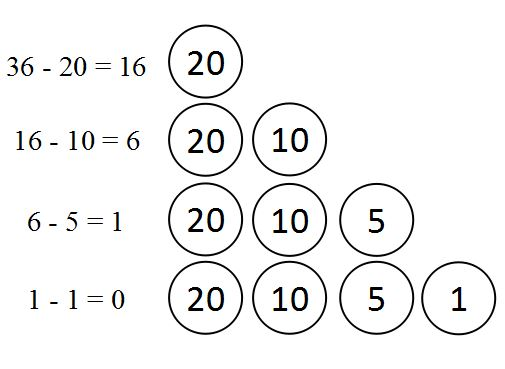
\includegraphics[width=8cm,height=8cm,keepaspectratio]{5.JPG}\\
\\Greedy algorithms determine minimum number of coins to give while making change. These are the steps a human would take to emulate a greedy algorithm to represent 36 cents using only coins with values {1, 5, 10, 20}. The coin of the highest value, less than the remaining change owed, is the local optimal.\\

With these in mind, the remainder of the paper is organized as follows. Section II discusses related works.Section III describes the definitions of  problem. Section IV and V presents formal model definitions and extended model definitions.  Section VI is the result of our simulation of MILP and greedy scheduler. Finally, Section VII concludes the paper.\\

\section{Related Works}
This section discusses some related works of DVFS, workflow scheduling and cluster computing.

%A. Reducing CPU energy cost
\subsection{ Reducing CPU energy cost}

In [3], the authors trying to saving energy by reducing CPU energy cost, they consider a new method for reducing the energy used by the CPU. Also, they introduce a new metric for CPU energy performance; millions-of-instructions-per-joule (MIPJ) which can be reduced by a class of methods like dynamic control of system clock speed by operating system scheduler.

So, they come up with some right scheduling algorithms for taking advantage of adjusting the clock speed at a fine grain, which CPU energy can be substantial saved with a limited impact on performance.

%B. Reduce the energy consumption of non-critical jobs
\subsection{Reduce the energy consumption of non-critical jobs}

In [1], the authors study the slack time for non-critical jobs, extends their execution time and reduces the energy consumption without increasing the task’s execution time as a whole. Moreover, they consider Green Service Level Agreement which is increasing task execution time within an affordable limit. They also develop a heuristic scheduling to reduce energy consumption of a tasks execution, and their main concern is discussing the relationship between energy consumption and task execution time.

%C. Case study of DVFS on processor clock frequencies at older and recent platform
\subsection{ Case study of DVFS on processor clock frequencies at older and recent platform}

In [2], the authors discuss how the clock frequency of a processor is decreased to allow a corresponding reduction in the supply voltage using Dynamic voltage and frequency scaling (DVFS). This power consumption reducing can lead to significant reduction in the energy for a computation, especially for memory-bound workloads. But that’s only for older platform; recent developments in processor and memory technology have brought in the saturation of processor clock frequencies. Then, they analysis how reduce processor clock frequency at DVFS on older and recent platforms. The result is that this method actually increases energy usage on most recent platforms; it can only effective on older platforms.

\subsection{ VM work placement to cut cost}
In [5], the paper study the multi-dimensonal resource usage states of physical machines. It talks about the problem of the natural imbalance of jobs to tend to favor a specific resource, such as CPU or memory. This results in jobs that fills up all phyiscal memory but very little CPU and vice versa. The paper proposes a set covering solutuion to reduce energy usage by using the minimal number of physical machines. This naturally results fitting the incoming jobs in such a way that packs high memory intensive jobs with high CPU intensive jobs. However, this solution is generally efficient and does not apply to workloads where you only have one type (CPU or Memory intensive workloads).\\

\section{Defintions}
% no \IEEEPARstart
First, we have the set of jobs, $J$:
$$J =\{j_1,j_2,j_3, ..., j_i\}$$

We also have the set of computing clusters (DVFS aware):
$$C =\{c_1,c_2,c_3, ..., c_j\}$$

Each DVFS cluster supports 2 energy states, taking from set $V$:
$$V =\{v_1,v_2\}$$

$v_1$ is used for non-critical jobs, $v_2$ is used for critical jobs. The notion of criticality is apparent throughout the relation between each sets. Essentially, noncritical jobs will get placed on noncritical clusters, which runs in noncritical energy state. Critical jobs will be ran on clusters that is of critical energy state $v_2$. Each cluster is either noncritical, or critical, and runs in the corresponding energy state.

We use a simple formula to calculate energy cost per job:\\

$TFT$: Task Finish Time\\
\indent $TST$: Task Starting Time\\

$\Omega = ($${{TFT_j}_i}$$ - $${{TST_j}_i}$$)*$${{p_v}_1}$$ $\\
\indent $\Omega = ($${{TFT_j}_i}$$ - $${{TST_j}_i}$$)*$${{p_v}_2}$$ $\\

The first term calculates the total execution time of job $j_i$ in $ms$, and the second term is $price$ $per$ $ms$ for voltage state $v_1$/$v_2$. $TFT$ and $TST$ are specified by the customer.

Last, we use two decision variables to denote whether a job is critical or noncritical:
$${{{{x_j}_i}_v}_1}\in \{0,1\}$$
$${{{{z_j}_i}_v}_2}\in \{0,1\}$$\\
Next, we will introduce our framework and talk about some specific considerations that is nonobvious and nontrivial.

\section{Model}
\subsection{Optimization}

min $\displaystyle{\sum \limits_{i=1}^{|J|} { (({TFT_j}_i} - {TST_j}_i)*{p_v}_1*{{{{x_j}_i}_v}_1})
+ (({TFT_j}_i} - {TST_j}_i)*{p_v}_2*{{{{z_j}_i}_v}_2) + (\epsilon_{penalty} * ms_{{penalty_j}_i}) }$\\

The first two terms simply calculate the energy cost of job $j_i$, while the last term is the penalty costs when job $j_i$ is not finished on time.

\subsection{Constraints}
(1) ${{{{x_j}_i}_v}_1} +{{{{z_j}_i}_v}_2} = 1$ for $ i = 1, 2, 3, ..., |J|$\\
\newline\indent Each job is either critical, or noncritical, but not both.\\
\newline\indent(2) $  ms_{{penalty_j}_i} \leq {TFT_j}_i - {TST_j}_i$ for $ i = 1, 2, 3, ..., |J|$\\
\newline\indent The penalty time should not be more than expected execution time. This also ensures each job gets scheduled and executed. If a job is not scheduled, then $ms_{{penalty_j}_i}$ is infinite.\\
% You must have at least 2 lines in the paragraph with the drop letter
% (should never be an issue)


% \hfill mds
 
% \hfill August 26, 2015

% \subsection{Subsection Heading Here}
% Subsection text here.


% \subsubsection{Subsubsection Heading Here}
% Subsubsection text here.


% An example of a floating figure using the graphicx package.
% Note that \label must occur AFTER (or within) \caption.
% For figures, \caption should occur after the \includegraphics.
% Note that IEEEtran v1.7 and later has special internal code that
% is designed to preserve the operation of \label within \caption
% even when the captionsoff option is in effect. However, because
% of issues like this, it may be the safest practice to put all your
% \label just after \caption rather than within \caption{}.
%
% Reminder: the "draftcls" or "draftclsnofoot", not "draft", class
% option should be used if it is desired that the figures are to be
% displayed while in draft mode.
%
%\begin{figure}[!t]
%\centering
%\includegraphics[width=2.5in]{myfigure}
% where an .eps filename suffix will be assumed under latex, 
% and a .pdf suffix will be assumed for pdflatex; or what has been declared
% via \DeclareGraphicsExtensions.
%\caption{Simulation results for the network.}
%\label{fig_sim}
%\end{figure}

% Note that the IEEE typically puts floats only at the top, even when this
% results in a large percentage of a column being occupied by floats.


% An example of a double column floating figure using two subfigures.
% (The subfig.sty package must be loaded for this to work.)
% The subfigure \label commands are set within each subfloat command,
% and the \label for the overall figure must come after \caption.
% \hfil is used as a separator to get equal spacing.
% Watch out that the combined width of all the subfigures on a 
% line do not exceed the text width or a line break will occur.
%
%\begin{figure*}[!t]
%\centering
%\subfloat[Case I]{\includegraphics[width=2.5in]{box}%
%\label{fig_first_case}}
%\hfil
%\subfloat[Case II]{\includegraphics[width=2.5in]{box}%
%\label{fig_second_case}}
%\caption{Simulation results for the network.}
%\label{fig_sim}
%\end{figure*}
%
% Note that often IEEE papers with subfigures do not employ subfigure
% captions (using the optional argument to \subfloat[]), but instead will
% reference/describe all of them (a), (b), etc., within the main caption.
% Be aware that for subfig.sty to generate the (a), (b), etc., subfigure
% labels, the optional argument to \subfloat must be present. If a
% subcaption is not desired, just leave its contents blank,
% e.g., \subfloat[].


% An example of a floating table. Note that, for IEEE style tables, the
% \caption command should come BEFORE the table and, given that table
% captions serve much like titles, are usually capitalized except for words
% such as a, an, and, as, at, but, by, for, in, nor, of, on, or, the, to
% and up, which are usually not capitalized unless they are the first or
% last word of the caption. Table text will default to \footnotesize as
% the IEEE normally uses this smaller font for tables.
% The \label must come after \caption as always.
%
%\begin{table}[!t]
%% increase table row spacing, adjust to taste
%\renewcommand{\arraystretch}{1.3}
% if using array.sty, it might be a good idea to tweak the value of
% \extrarowheight as needed to properly center the text within the cells
%\caption{An Example of a Table}
%\label{table_example}
%\centering
%% Some packages, such as MDW tools, offer better commands for making tables
%% than the plain LaTeX2e tabular which is used here.
%\begin{tabular}{|c||c|}
%\hline
%One & Two\\
%\hline
%Three & Four\\
%\hline
%\end{tabular}
%\end{table}


% Note that the IEEE does not put floats in the very first column
% - or typically anywhere on the first page for that matter. Also,
% in-text middle ("here") positioning is typically not used, but it
% is allowed and encouraged for Computer Society conferences (but
% not Computer Society journals). Most IEEE journals/conferences use
% top floats exclusively. 
% Note that, LaTeX2e, unlike IEEE journals/conferences, places
% footnotes above bottom floats. This can be corrected via the
% \fnbelowfloat command of the stfloats package.

\section{Extended Model}

In addition, we include an incoming jobs queue for the set $$J =\{j_1,j_2,j_3, ..., j_i\}$$
These incoming jobs will first be stored in a centralized queue.\\\\
% scheduler queue picture below
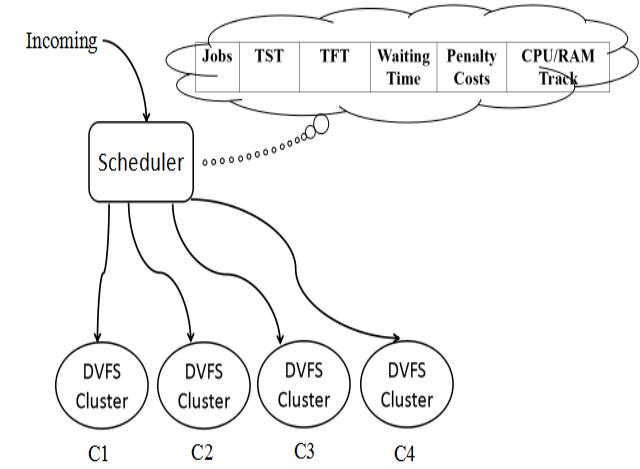
\includegraphics[width=9.8cm,height=26.8cm,keepaspectratio]{1-g.JPG}\\
\\Using greedy algorithm, the scheduler allocate jobs to low energy cluster first. At each step we pick the jobs with the earliest deadline. The general goal that we will try to sqeeze all jobs into low energy cluster and only use high energy cluster when certain $threshold$ are reached. In essense, if it is possible to finish all tasks without resorting to use of more expensive resources, then we will take that path.\\\\
% low queue
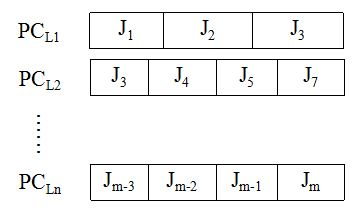
\includegraphics[width=8cm,height=8cm,keepaspectratio]{2.JPG}\\
\\First, we will sort the incoming job queue $J$ in ascending deadline:
$${j_1}_{deadline} \leq {j_2}_{deadline} \leq {j_3}_{deadline} \leq ... \leq {j_n}_{deadline}$$

If there are many jobs have the same deadline at our centralized queue. We execute them in their order at our queue (FIFO). The sorting facilitates our greedy scheduling algorithm.

If there are one or more jobs that extend past their respective deadlines and also cross over the $threshold$, then the set of those jobs is transfered to a high energy cluster queue(s). If there are no available resources to take on those jobs, then that set of jobs will wait in queue.

% high queue
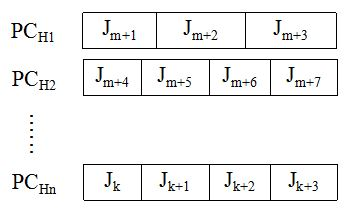
\includegraphics[width=8cm,height=8cm,keepaspectratio]{3.JPG}\\
\\At the next scheduling period, we will make another determination to see if any high energy clusters are available to take on those jobs. While in queues and during execution, the jobs may accumlate deadline cost penalities. Thus, in the $threshold$ for decision making, as mentioned before, will include two variables. The first variable is the penality cost accured, and the second variable is the data transfer cost. 
\\
\\penalty cost = data transfer cost + $\sum \limits_{i=1}^{|J|} (\epsilon_{penalty} * ms_{{penalty_j}_i})$\\
\newline
The data transfer cost is simply the cost resulting from the fact that transfering a job from low energy to a high energy cluster results in a time delay. That delay can be thought of as an increase in expected executation time of the job. Generally, if the transfer time is more than the time gained by switching from a low energy cluster to a high energy cluster, then we should reject switching to a high energy cluster. Each job's expected executation is intitally calculated as follows.
$${j_i}_{execution} = \frac{CPI*Instruction Count}{Processor Frequency}$$ 

It is calculated twice, once for low energy cluster and once for higher energy cluster.

But, there is still an important issue, if a random job ${j_r}_{deadline}$ has a relatively later deadline, and new jobs with earlier deadlines keep coming into our centralized queue, that will cause a big problem, which is keeping this random job $j_r$ in our queue for a long time, thus will have a negative influence at user experience. So, the variable "waiting time" is used to let those jobs we mentioned before have a high priority at our centralized queue, and can be executed first. When the waiting time of a random job $j_r$ is higher or equal to its execution time, we promote a high priority to this job $j_r$ . If there are two jobs have been promoting a high priority and have the same waiting time and execution time which equals "deadline minus enter time", then we execute them in their order at centralized queue.\\

\section{Results}
In our testing, we use Microsoft Azure cloud and rented 35 computers to test three workload types. The first type is a typical workload, which consist of an mixed amount of memory, storage, and CPU intensive jobs. The second type is CPU bound jobs. This job type is also fairly common among cloud computing jobs. The last type is memory intensive jobs, to represent jobs like MapReduce. We compare our scheduler to 2 other typical industry schedulers.\\
\newline
% high queue
\includegraphics[width=8.8cm,height=8.8cm,keepaspectratio]{graph1.png}\\\\
Mixed workload shows our scheduler outperforming the other two scheduler.\\\\
\newline
% high queue
\includegraphics[width=8.8cm,height=8.8cm,keepaspectratio]{graph2.png}\\\\
Under CPU bound workload conditions, all schedulers show similar performance.\\\\
\newline
% high queue
\includegraphics[width=8.8cm,height=8.8cm,keepaspectratio]{graph3.png}\\\\
Again, all schedulers demonstrate similar performance.\\
\section{Conclusion}
Our scheduling method demonstrates moderate improvments when dealing with CPU intensive jobs and mixed jobs workloads. This is reflected in the fact that in a worload of 40 jobs, our scheduling method used the least amount of computing resource. This is already a cost improvement since idle resouces can be used to run more jobs or turned off to further improve power use. In the case of CPU bound job types, our scheduling method showed a small improvement, but this is expected as energy saving is diffculty when a great amount of CPU resource is required for proper execution of a job. In the last type of jobs, all scheduling methods show very similar results. This is also expected. Moreover, our scheduling method did not attempt to minimize memory or network usage.




% conference papers do not normally have an appendix


% use section* for acknowledgment
%\section*{Acknowledgment}



%placeholder.





% trigger a \newpage just before the given reference
% number - used to balance the columns on the last page
% adjust value as needed - may need to be readjusted if
% the document is modified later
%\IEEEtriggeratref{8}
% The "triggered" command can be changed if desired:
%\IEEEtriggercmd{\enlargethispage{-5in}}

% references section

% can use a bibliography generated by BibTeX as a .bbl file
% BibTeX documentation can be easily obtained at:
% http://mirror.ctan.org/biblio/bibtex/contrib/doc/
% The IEEEtran BibTeX style support page is at:
% http://www.michaelshell.org/tex/ieeetran/bibtex/
%\bibliographystyle{IEEEtran}
% argument is your BibTeX string definitions and bibliography database(s)
%\bibliography{IEEEabrv,../bib/paper}
%
% <OR> manually copy in the resultant .bbl file
% set second argument of \begin to the number of references
% (used to reserve space for the reference number labels box)
\begin{thebibliography}{1}

\bibitem{IEEEhowto:kopka}
Wang, Lizhe, et al. "Towards energy aware scheduling for precedence constrained parallel tasks in a cluster with DVFS." Cluster, Cloud and Grid Computing (CCGrid), 2010 10th IEEE/ACM International Conference on. IEEE, 2010.

\bibitem{IEEEhowto:kopka}
Le Sueur, Etienne, and Gernot Heiser. "Dynamic voltage and frequency scaling: The laws of diminishing returns." Proceedings of the 2010 international conference on Power aware computing and systems. 2010.

\bibitem{IEEEhowto:kopka}
Weiser, Mark, Brent Welch, Alan Demers, and Scott Shenker. "Scheduling for reduced CPU energy." In Mobile Computing, pp. 449-471. Springer US, 1994.

\bibitem{IEEEhowto:kopka}
Ren, Shaolei, Yuxiong He, and Fei Xu. "Provably-efficient job scheduling for energy and fairness in geographically distributed data centers." Distributed Computing Systems (ICDCS), 2012 IEEE 32nd International Conference on. IEEE, 2012.

\bibitem{IEEEhowto:kopka}
[5] Li, Xin, et al. "Energy efficient virtual machine placement algorithm with balanced and improved resource utilization in a data center." Mathematical and Computer Modelling 58.5 (2013): 1222-1235.

\end{thebibliography}




% that's all folks
\end{document}


